\documentclass{article}

\author{Artur Amaral}
\title{EEL480 - Laboratório de Sistemas Digitais Relatório 01}

\usepackage[T1]{fontenc}
\usepackage{listings}
\usepackage[utf8]{inputenc}
\usepackage[portuguese]{babel}
\usepackage{hyphenat}
\hyphenation{mate-mática recu-perar}
\usepackage{graphicx}

% Pendências:
% - Comentar bloco da ALU.


\begin{document}

\maketitle

\section{Introdução}

    O seguinte relatório descreve a implementação de uma unidade lógica e aritmética
em linguagem VHDL. Para escrita e teste do código, utilizou-se o software de
desenvolvimento Quartus II Lite, da Intel. O projeto final foi aplicado em uma
placa de prototipagem FPGA Altera DE2-115, cuja configuração é feita
remotamente pelo serviço online Labsland.

Além da ALU, o projeto consiste em um módulo bancada de testes, que gera,
através de um contador de 8 bits, entradas para a unidade, bem como em módulos
decodificadores hexadecimal para display de 7 segmentos, facilitando a visualização
dos dados durante o teste.

\section{Desenvolvimento do projeto}

\subsection{Especificações iniciais}

\begin{itemize}
    \item Dois operandos hexadecimais  X e Y de 4 bits.
    \item Uma saída hexadecimal Z de 4 bits.
    \item Uma entrada de seleção S de 3 bits, permitindo 8 operações.
    \item Faixa de valores representada:
        \begin{itemize}
            \item  0 <= X, Y <= 15
            \item  -15 <= Z <= 15
        \end{itemize}
    \item 4 Flags (LEDs): Negativo, Zero, Overflow, Carry Out.
    \item Obs: As Flags só possuem sentido explícito nas operações de adição e subtração.
\end{itemize}


\subsection{Tabela de operações}

\begin{center}
    \begin{tabular}{ c|c|c }

        \textbf{Seleção} & \textbf{Operação} & \textbf{Descrição} \\
    000 & RESET & Força zero\\
    001 & X MAIS Y & Adição\\
    010 & X MENOS Y & Subtração\\
    011 & X AND Y & And bit a bit\\
    100 & X OR Y & Or bit a bit\\
    101 & X XOR Y & Xor bit a bit\\
    110 & NOT X & Not bit a bit\\
    111 & PRESET & Força um\\

\end{tabular}
\end{center}

\begin{verbatim}
\end{verbatim}


\begin{center}
\textbf{Diagrama de blocos da ALU}
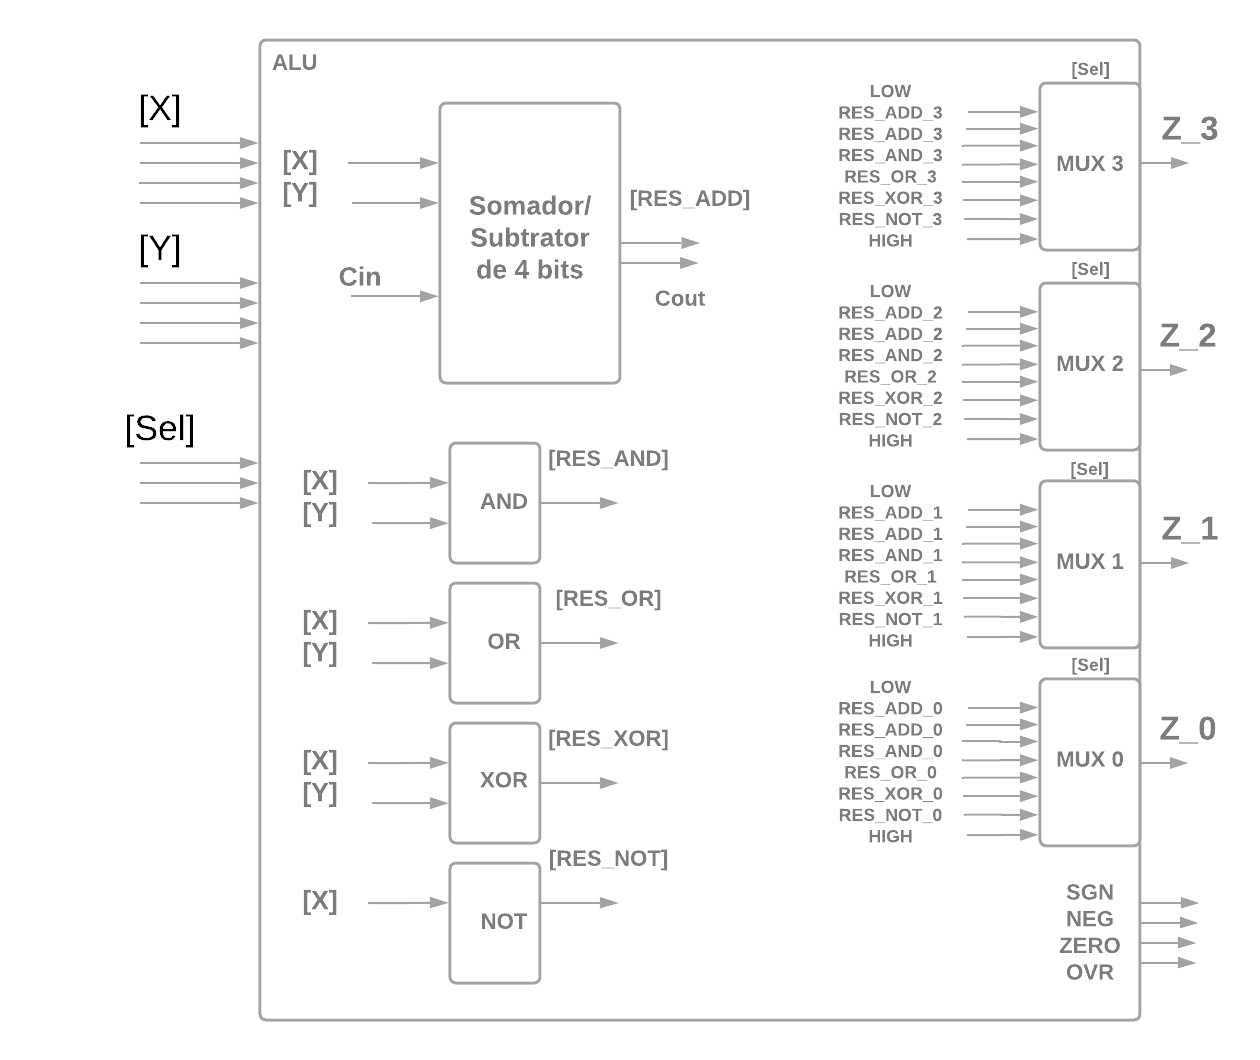
\includegraphics[width=\textwidth]{img/DB_ALU.png}
\textbf{Diagrama de blocos da bancada de testes}
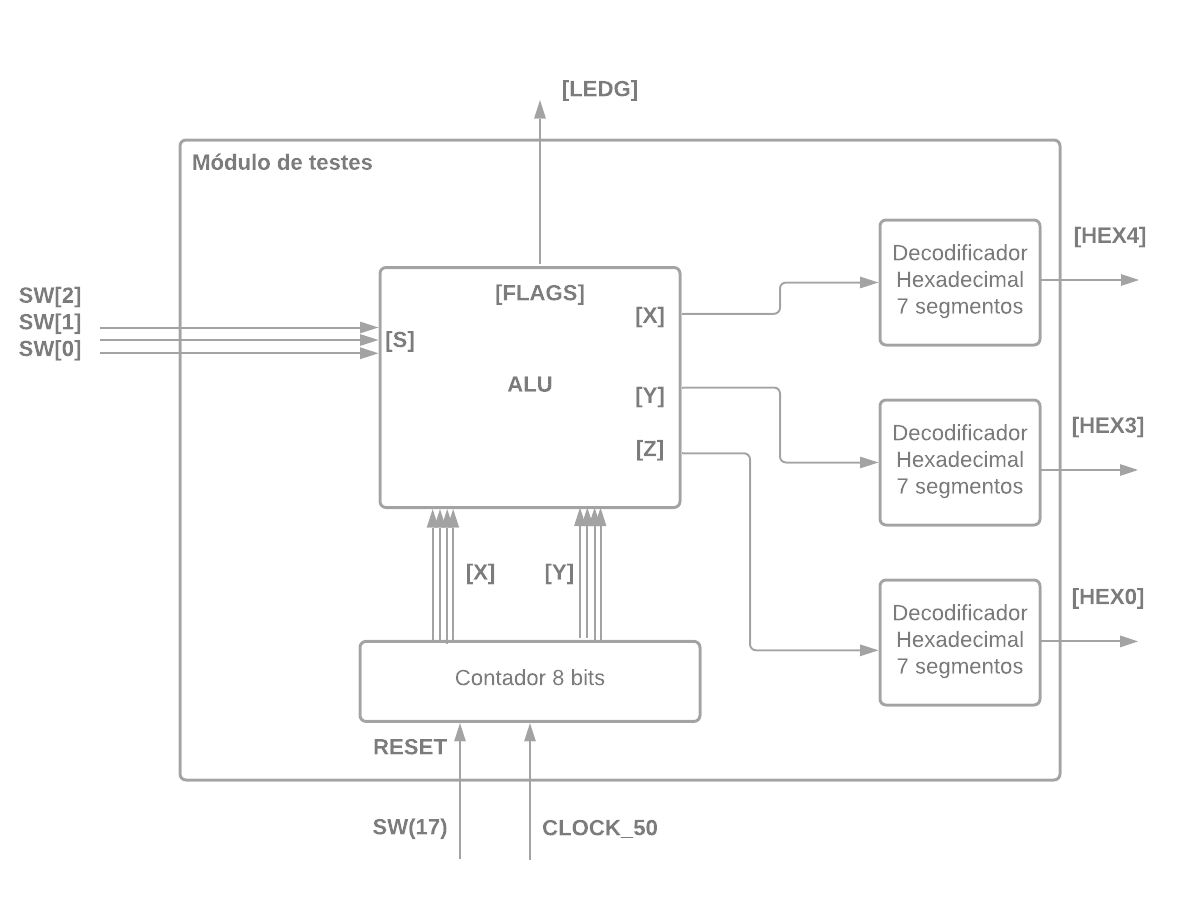
\includegraphics[width=\textwidth]{img/DB_Teste.png}
\end{center}

\subsection{Modularização em VHDL / Hierarquia dos arquivos}

Cada bloco representado nos diagramas acima equivale a um arquivo vhd do código,
formando diferentes componentes que se relacionam através de uma hierarquia.

Um componente estar abaixo de outro na hierarquia significa que aquele foi
incluso no código deste, e consiste de um bloco independente e funcional, mas
que exerce uma função relevante ao bloco externo.

\begin{verbatim}
ALU_testbench.vhd
|
|_counter_8bits.vhd
|_hex_to_display.vhd
|_ALU.vhd
   |
   |_addSub4bits.vhd
       |_fullAdder.vhd
   |_and4bits.vhd
   |_or4bits.vhd
   |_xor4bits.vhd
   |_not4bits.vhd
   |_mux_8_to_1.vhd

\end{verbatim}

\subsection{Implementação em VHDL dos módulos}

Nesta seção, serão apresentadas as implementações em VHDL de cada um dos módulos,
com a inserção de comentários explicativos quando for relevante. Os módulos são
apresentados na ordem cronológica em que foram desenvolvidos, naturalmente partindo
dos blocos de menor para os de maior complexidade.

Para ilustrar, em alguns módulos serão expostas fotos de simulações realizadas no
Quatus, que validam seu funcionamento individual.
\newline

\textbf{Módulo AND}

\begin{verbatim}


library IEEE;
use IEEE.std_logic_1164.all;

entity and4bits is

port (
	a, b : in std_logic_vector(3 downto 0);
	s : out std_logic_vector(3 downto 0)
);

end and4bits;

architecture hardware of and4bits is
begin
	s <= a and b;
end hardware;

\end{verbatim}

\textbf{Módulo OR}

\begin{verbatim}


library IEEE;
use IEEE.std_logic_1164.all;

entity or4bits is

port (
	a, b : in std_logic_vector(3 downto 0);
	s : out std_logic_vector(3 downto 0)
);

end or4bits;

architecture hardware of or4bits is
begin
	s <= a or b;
end hardware;

\end{verbatim}

\textbf{Módulo XOR}

\begin{verbatim}


library IEEE;
use IEEE.std_logic_1164.all;

entity xor4bits is

port ( 
	a, b : in std_logic_vector(3 downto 0);
	s : out std_logic_vector(3 downto 0)
);

end xor4bits;

architecture hardware of xor4bits is
begin
	s <= a xor b;
end hardware;

\end{verbatim}

\textbf{Módulo NOT}

\begin{verbatim}

library IEEE;
use IEEE.std_logic_1164.all;

entity not4bits is

port (
	a : in std_logic_vector(3 downto 0);
	s : out std_logic_vector(3 downto 0)
);

end not4bits;

architecture hardware of not4bits is
begin
	s <= not a;
end hardware;

\end{verbatim}

\textbf{Módulo full adder}
\newline

Para a implementação do somador, criou-se primeiro um módulo full adder, que
realiza uma soma de 1 bit. Então, o somador de 4 bits consiste de uma 
composição de 4 full adders.

\begin{verbatim}

library IEEE;
use IEEE.std_logic_1164.all;


entity fullAdder is

port (
	a, b, cin : in std_logic;
	s, cout : out std_logic
);

end fullAdder;

architecture hardware of fullAdder is
begin
	s <= a xor b xor cin;
	cout <= (b and cin) or (a and cin) or (a and b);
end hardware;

\end{verbatim}

\textbf{Módulo somador subtrator}
\newline

Este somador implementa uma subtração quando recebe um carry in, que depende
da entrada de seleção da ALU. O que acontece é que o operando Y é complementado
de 2 e então somado. Este módulo segue o seguinte esquema: 


\begin{center}
\begin{figure}
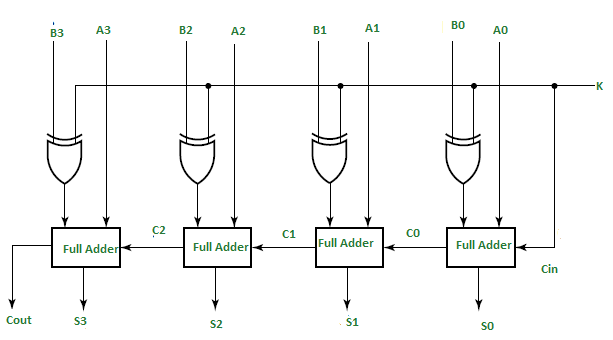
\includegraphics[width=0.8\textwidth]{img/AddSub4bits.png}
\caption{Retirado de: https://www.geeksforgeeks.org/4-bit-binary-adder-subtractor/ }
\end{figure}
\end{center}

\begin{verbatim}

library IEEE;
use IEEE.std_logic_1164.all;

entity addSub4bits is
port (
	A, Bin : in std_logic_vector(3 downto 0);
	S : 		out std_logic_vector(3 downto 0);
	CIN : 	in std_logic;
	COUT : 	out std_logic
);

end addSub4bits;

architecture hardware of addSub4bits is

-- Instanciação do componente fulladder para uso do somator/subtrator de 4 bits.
-- Descreve a interface deste submódulo para uso externo a ele

component fullAdder is 

port (
	a, b, cin : in std_logic;
	s, cout : out std_logic
);

end component;
	
	-- Declaração de sinais.
	-- C é um vetor que descreve todos os carrys do componente.
	-- Bout é a saída da entrada
	
	signal C : std_logic_vector (4 downto 0);
	signal Bout : std_logic_vector (3 downto 0);

begin

gen: for i in 0 to 3 generate

	Bout(i) <= Bin(i) XOR CIN;

	FA: fullAdder port map(a=>A(i), b => Bout(i), cin => C(i), s => S(i), cout => C(i+1)); 

end generate;

C(0) <= CIN;
COUT <= C(4);
	
end hardware;

\end{verbatim}

\textbf{Módulo NOT}

\begin{verbatim}

library IEEE;
use IEEE.std_logic_1164.all;

entity mux_8_to_1 is

port (
	a : in std_logic_vector(7 downto 0);
	s : in std_logic_vector(2 downto 0);
	o : out std_logic
);
end mux_8_to_1;

architecture hardware of mux_8_to_1 is
begin
process(a,s)
begin

	o <= '0';
	
	case s is
		when "000" => o <= a (0);
		when "001" => o <= a (1);
		when "010" => o <= a (2);
		when "011" => o <= a (3);
		when "100" => o <= a (4);
		when "101" => o <= a (5);
		when "110" => o <= a (6);
		when "111" => o <= a (7);
		when others => o <= '0';
	end case;

end process;
end hardware;

\end{verbatim}

\begin{center}
\textbf{Teste multiplexador}
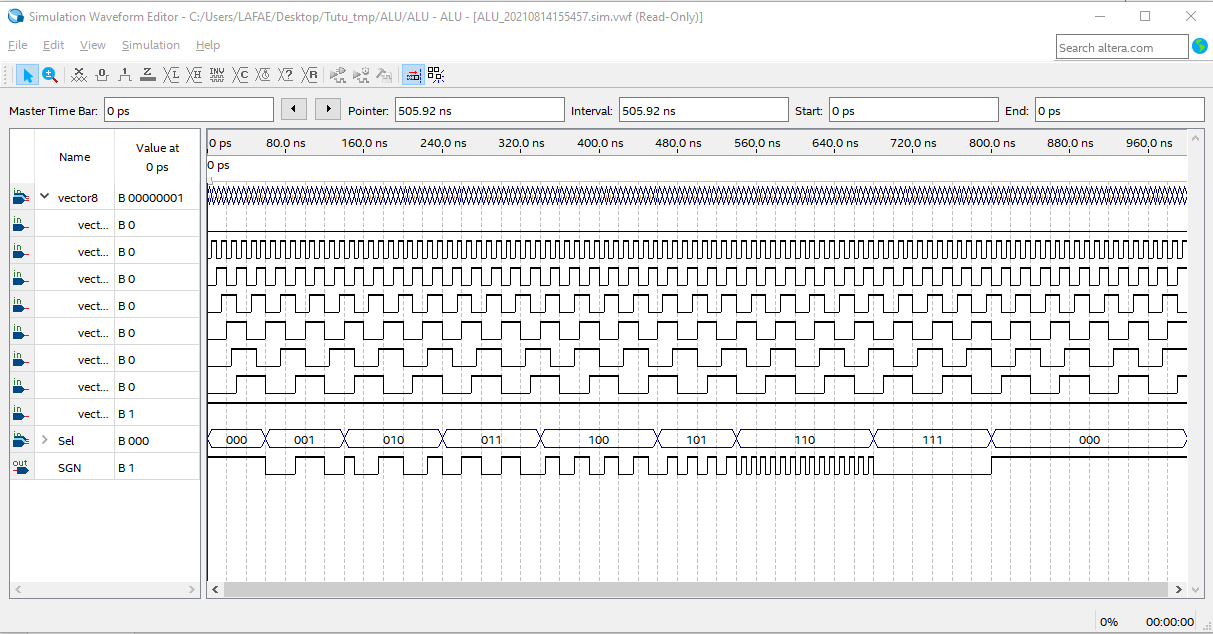
\includegraphics[width=\textwidth]{img/teste_mux.png}
\end{center}



\textbf{Módulo ALU}

\begin{verbatim}

library IEEE;
use IEEE.std_logic_1164.all;

-----------------------------------
-- Descrição da interface da ALU -- 
-----------------------------------
entity ALU is 
port (
	X, Y : in std_logic_vector(3 downto 0);
	Sel : in std_logic_vector(2 downto 0);
	Z : buffer std_logic_vector(3 downto 0);
	NEG, ZERO, OVR : out std_logic;
	Cout : buffer std_logic
);

end ALU;

-------------------------------------
-- Descrição da arquitetura da ALU -- 
-------------------------------------
architecture hardware of ALU is

----------------------------------------
-- Importação de componentes externos --
----------------------------------------

------------------------------------------
-- Módulo de adição/subtração de 4 bits --
------------------------------------------
component addSub4bits is 
port (
	A, Bin : in std_logic_vector(3 downto 0);
	S : 		out std_logic_vector(3 downto 0);
	CIN : 	in std_logic;
	COUT : 	out std_logic
);
end component;

--------------------------
-- Módulo AND de 4 bits --
--------------------------
component and4bits is 
port(
	a, b : in std_logic_vector(3 downto 0);
	s : out std_logic_vector(3 downto 0)
);
end component;

-------------------------
-- Módulo OR de 4 bits --
-------------------------
component or4bits is 
port(
	a, b : in std_logic_vector(3 downto 0);
	s : out std_logic_vector(3 downto 0)
);
end component;

--------------------------
-- Módulo XOR de 4 bits --
--------------------------
component xor4bits is 
port(
	a, b : in std_logic_vector(3 downto 0);
	s : out std_logic_vector(3 downto 0)
);
end component;

--------------------------
-- Módulo NOT de 4 bits --
--------------------------
component not4bits is
port (
	a : in std_logic_vector(3 downto 0);
	s : out std_logic_vector(3 downto 0)
);
end component;

--------------------------
-- Módulo multiplexador -- 
--------------------------
component mux_8_to_1 is
port (
	a : in std_logic_vector(7 downto 0);
	s : in std_logic_vector(2 downto 0);
	o : out std_logic
);
end component;
	
	signal res_reset : std_logic_vector(3 downto 0);
	signal res_addSub : std_logic_vector(3 downto 0); 
	signal res_and: std_logic_vector(3 downto 0);
	signal res_or:	std_logic_vector(3 downto 0);
	signal res_xor: std_logic_vector(3 downto 0);
	signal res_not: std_logic_vector(3 downto 0);
	signal res_preset : std_logic_vector(3 downto 0);
	signal Cout_internal : std_logic;

begin
	
	opAddSub: addSub4bits port map(A => X, Bin => Y, CIN =>Sel(1),
                            S=>res_addSub, COUT=> Cout_internal);
	opAnd: and4bits port map(a=>X, b=>Y, s=>res_and);
	opOr: or4bits port map(a=>X, b=>Y, s=>res_or);
	opXor: xor4bits port map(a=>X, b=>Y, s=>res_xor);
	opNot: not4bits port map(a=>X, s=>res_not);
	
	-- Nesse caso, i representa o número do mux, que dão as saídas da
	-- ALU. O mux zero emite a saída z0, LSB, e assim por diante.
	
	gen: for i in 0 to 3 generate
		mux: mux_8_to_1 port map(
				a(0) => res_reset(i),
				a(1) => res_addSub(i),
				a(2) => res_addSub(i),
				a(3) => res_and(i),
				a(4) => res_or(i),
				a(5) => res_xor(i),
				a(6) => res_not(i),
				a(7) => res_preset(i),
				s=>Sel,
				o=>Z(i)
			);
	end generate;
	
	res_reset <= "0000";
	res_preset <= "1111";
	
	Cout <= Cout_internal and (((not Z(2)) and (not Z(1)) and Z(0)) or 
                                ((not Z(2)) and Z(1) and (not Z(0)))); 

	ZERO <= not (Z(0) or Z(1) or Z(2) or Z(3));

-- O número apenas é negativo em caso de subtração, logo a condição é Cout=0 E S=010.
NEG <= (not Cout) and (not Sel(2)) and Sel(1) and (not Sel(0));

-- Overflow só existe em caso de soma na minha ALU, logo há OVR quando há Cout=1 E S=001.
OVR <= Cout and ( (not Sel(2)) and (not Sel(1)) and Sel(0) ); 	

end architecture;

\end{verbatim}

\textbf{Módulo Contador de 8 bits}
\newline

Dos 8 bits gerados por esse contador, os 4 menos significativos compoem X e os 
4 mais significativos, Y.

Vale notar que há um divisor de frequência neste módulo. Como clock recebido é de 
50 Mhz, esta frequência foi dividida por 100 milhões, o que gera um período de
contagem da ordem de 2 segundos.

\begin{verbatim}

library IEEE;
use IEEE.std_logic_1164.all;
use IEEE.numeric_std.all;
use IEEE.std_logic_unsigned.all;

entity counter_8bits is 
port (

	Reset : in std_logic;
	Clock : in std_logic;
	Counter_output : out std_logic_vector(7 downto 0)

);
end counter_8bits;

architecture hardware of counter_8bits is 

signal counter : std_logic_vector (7 downto 0);

begin

process(Reset, Clock)

variable clockCount : std_logic_vector (30 downto 0) := (others=>'0');

begin

	if Reset='1' then
		clockCount := (others=>'0');
	elsif (Clock'event and Clock = '1') then
		clockCount := clockCount + 1;
		
		if (clockCount = 100000000) then
			clockCount :=  (others=>'0');
			counter <= counter + 1;
		end if;
		
	end if;
	
end process;

-- Mude essa atribuição para revezar entre clock e contagem em segundos.
Counter_output <= counter; 

end hardware;

\end{verbatim}


\begin{center}
\textbf{Teste contador 8 bits}
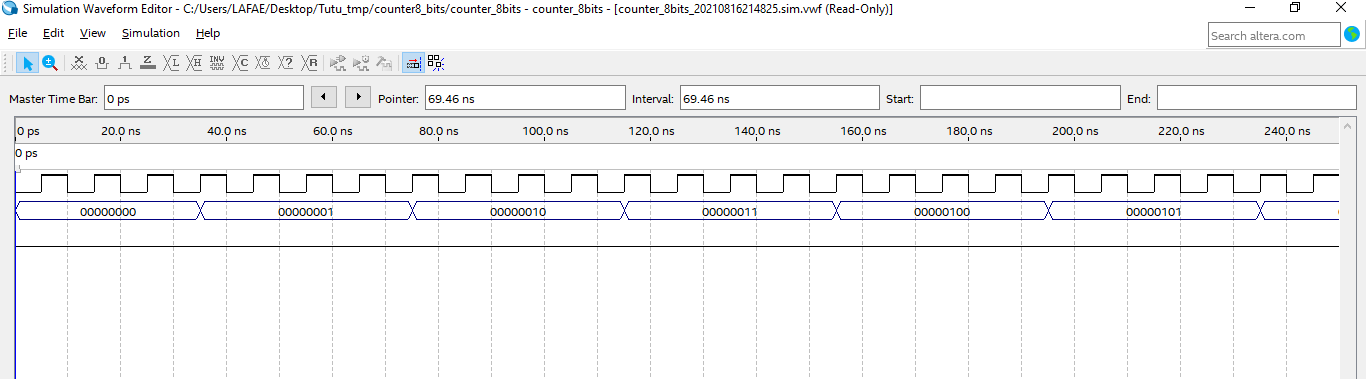
\includegraphics[width=\textwidth]{img/teste_contador.png}
\end{center}


\textbf{Módulo decodificador hexadecimal 7 segmentos}

\begin{verbatim}

library IEEE;
use IEEE.std_logic_1164.all;

entity hex_to_display is 

port (
	
	hex : in std_logic_vector(3 downto 0);
	display : out std_logic_vector(6 downto 0)

);
end hex_to_display;

architecture hardware of hex_to_display is

begin

process(hex)
begin

	case hex is
	
		when "0000" => display <= "1000000";
		when "0001" => display <= "1111001";
		when "0010" => display <= "0100100";
		when "0011" => display <= "0110000";
		when "0100" => display <= "0011001";
		when "0101" => display <= "0010010";
		when "0110" => display <= "0000010";
		when "0111" => display <= "1111000";
		when "1000" => display <= "0000000";
		when "1001" => display <= "0011000";
		when "1010" => display <= "0001000";
		when "1011" => display <= "0000011";
		when "1100" => display <= "1000110";
		when "1101" => display <= "0100001";
		when "1110" => display <= "0000110";
		when "1111" => display <= "0001110";
		
	end case;
		
end process;



end hardware;

\end{verbatim}

\textbf{Módulo bancada de testes}

\begin{verbatim}

library IEEE;
use IEEE.std_logic_1164.all;

entity alu_testbench is
port(
	HEX4 : out std_logic_vector(6 downto 0);
    HEX3 : out std_logic_vector(6 downto 0);
	HEX1 : out std_logic_vector(6 downto 0);
	SW: in std_logic_vector(17 downto 0);
	LEDG: out std_logic_vector(17 downto 0);
	CLOCK_50: in std_logic
);
end alu_testbench;

architecture hardware of alu_testbench is

component alu is
port (
	X, Y : in std_logic_vector(3 downto 0);
	Sel : in std_logic_vector(2 downto 0);
	Z : buffer std_logic_vector(3 downto 0);
	NEG, ZERO, OVR : out std_logic;
	Cout : buffer std_logic
);
end component;

component counter_8bits is
port (
	Reset : in std_logic;
	Clock : in std_logic;
	Counter_output : out std_logic_vector(7 downto 0)
);
end component;

component hex_to_display is
port (
	hex : in std_logic_vector(3 downto 0);
	display : out std_logic_vector(6 downto 0)
);
end component;

	signal t_X :  std_logic_vector(3 downto 0);
	signal t_Y :  std_logic_vector(3 downto 0);
	signal t_Sel :  std_logic_vector(2 downto 0);
	signal t_Z :  std_logic_vector(3 downto 0);
	signal t_NEG, t_ZERO, t_OVR, t_Cout : std_logic;
	
	
	signal in_decod_x : std_logic_vector(3 downto 0);
	signal out_decod_x : std_logic_vector(6 downto 0);
	
	signal in_decod_y : std_logic_vector(3 downto 0);
	signal out_decod_y : std_logic_vector(6 downto 0);
	
	signal in_decod_Z : std_logic_vector(3 downto 0);
	signal out_decod_Z : std_logic_vector(6 downto 0);
	
	signal t_reset : std_logic;
	signal t_Counter_output: std_logic_vector (7 downto 0);
	
begin

	alu_module: alu port map(X => t_X, Y => t_Y, Sel => t_Sel, Z => t_Z,
                            NEG => t_NEG, ZERO => t_ZERO,
                            OVR => t_OVR, Cout => t_Cout);
	display_decoder_x: hex_to_display port map(hex => t_X, display => out_decod_x);
	display_decoder_y: hex_to_display port map(hex => t_Y, display => out_decod_y);
	display_decoder_z: hex_to_display port map(hex => t_Z, display => out_decod_z);
	counter: counter_8bits port map(Reset => t_Reset, Clock => CLOCK_50,
                                    Counter_output => t_Counter_output);
	
	t_Sel (2) <= SW(2);
	t_Sel (1) <= SW(1);
	t_Sel (0) <= SW(0);
	
	gen0: for i in 0 to 3 generate
		t_X(i) <=  t_Counter_output(i);
	end generate;
	gen1: for i in 4 to 7 generate
		t_Y(i-4) <= t_Counter_output(i);
	end generate;
	
	in_decod_x <= t_X;
	in_decod_x <= t_Y;
	in_decod_x <= t_Z;
	
	HEX4 <= out_decod_x;
	HEX3 <= out_decod_y;
	HEX1 <= out_decod_z;
	
	LEDG(3) <= t_NEG;
	LEDG(2) <= t_ZERO;
	LEDG(1) <= t_OVR;
	LEDG(0) <= t_Cout;
	
	
end hardware; 

\end{verbatim}

\begin{center}
\textbf{Teste ALU com contador}
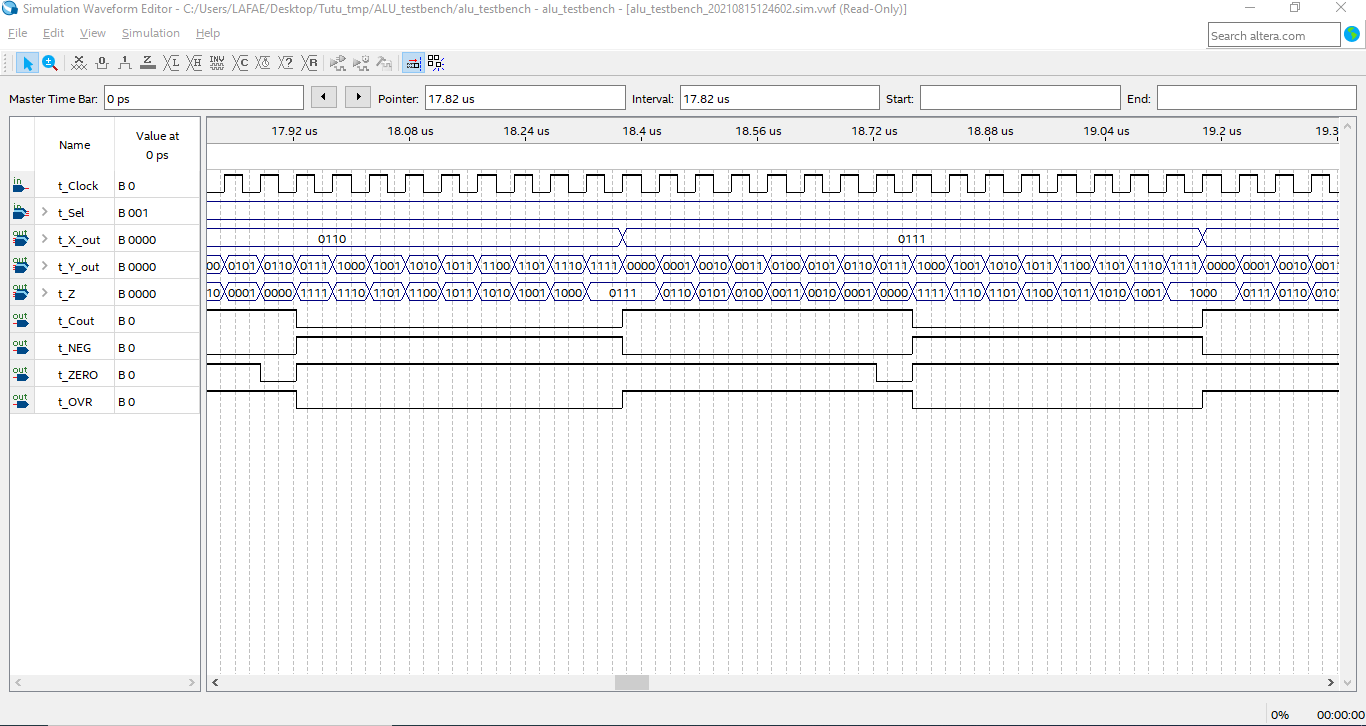
\includegraphics[width=\textwidth]{img/teste_alu_com_contador.png}
\end{center}

\section{Snapshots do funcionamento no LABSLAND}

\begin{center}

\begin{figure}
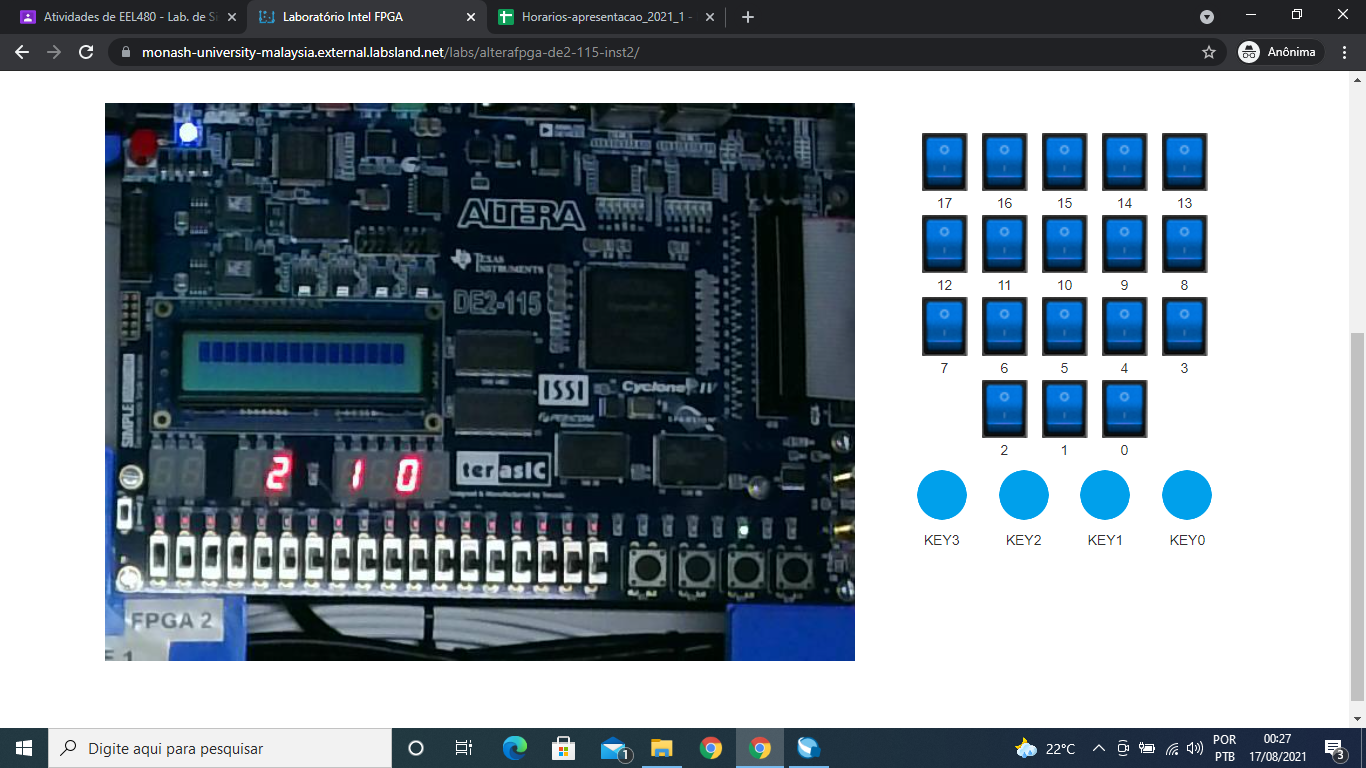
\includegraphics[width=\textwidth]{img/labsland_forca_zero.png}
\caption{Força zero}
\end{figure}

\begin{figure}
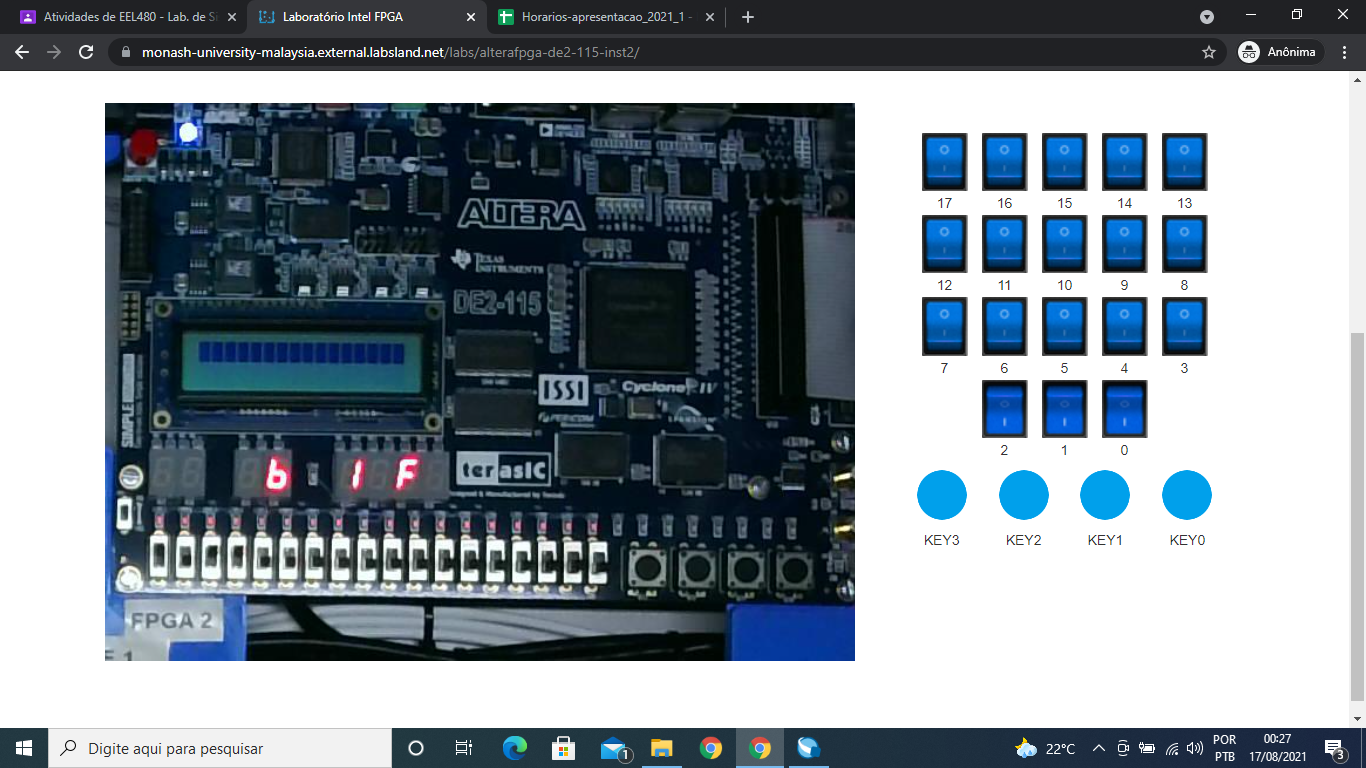
\includegraphics[width=\textwidth]{img/labsland_forca_1.png}
\caption{Força um}
\end{figure}

\begin{figure}
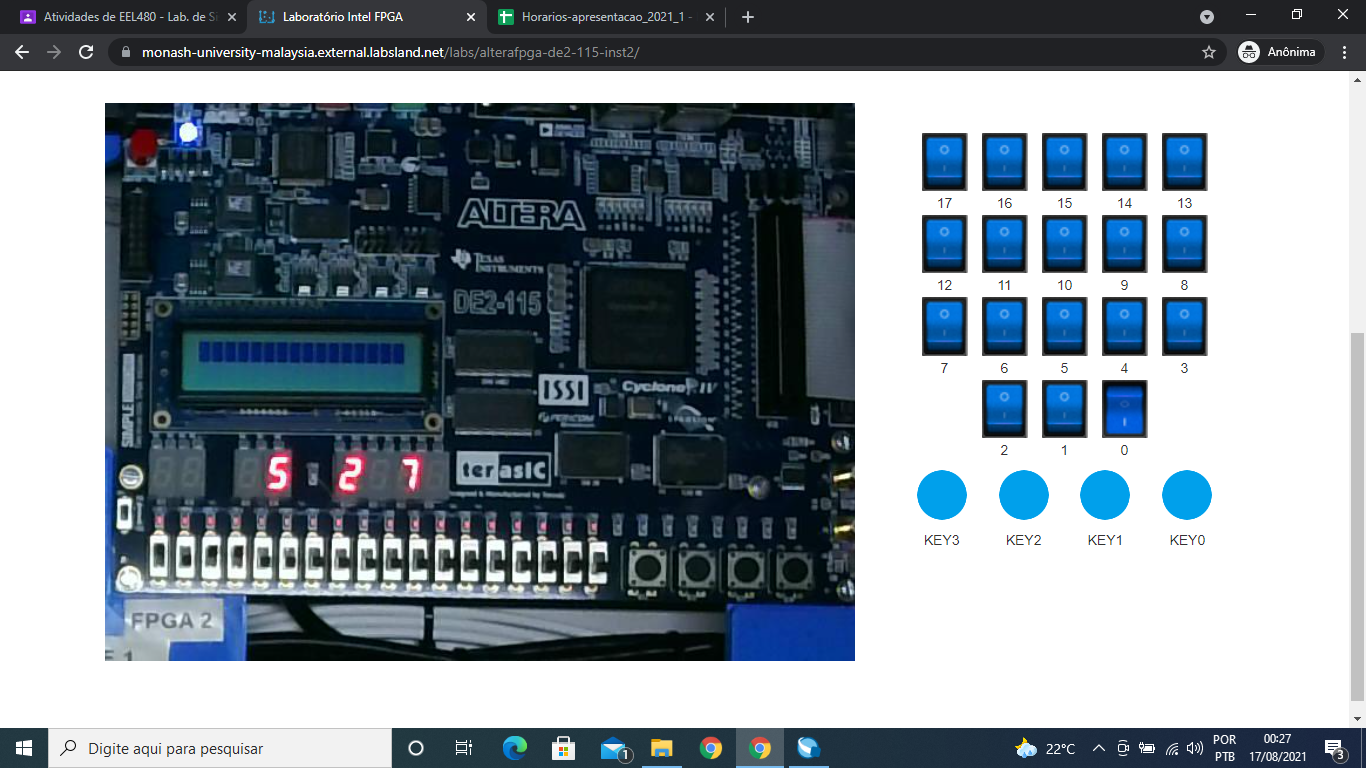
\includegraphics[width=\textwidth]{img/labsland_soma.png}
\caption{Soma: 5 + 2 = 7}
\end{figure}

\begin{figure}
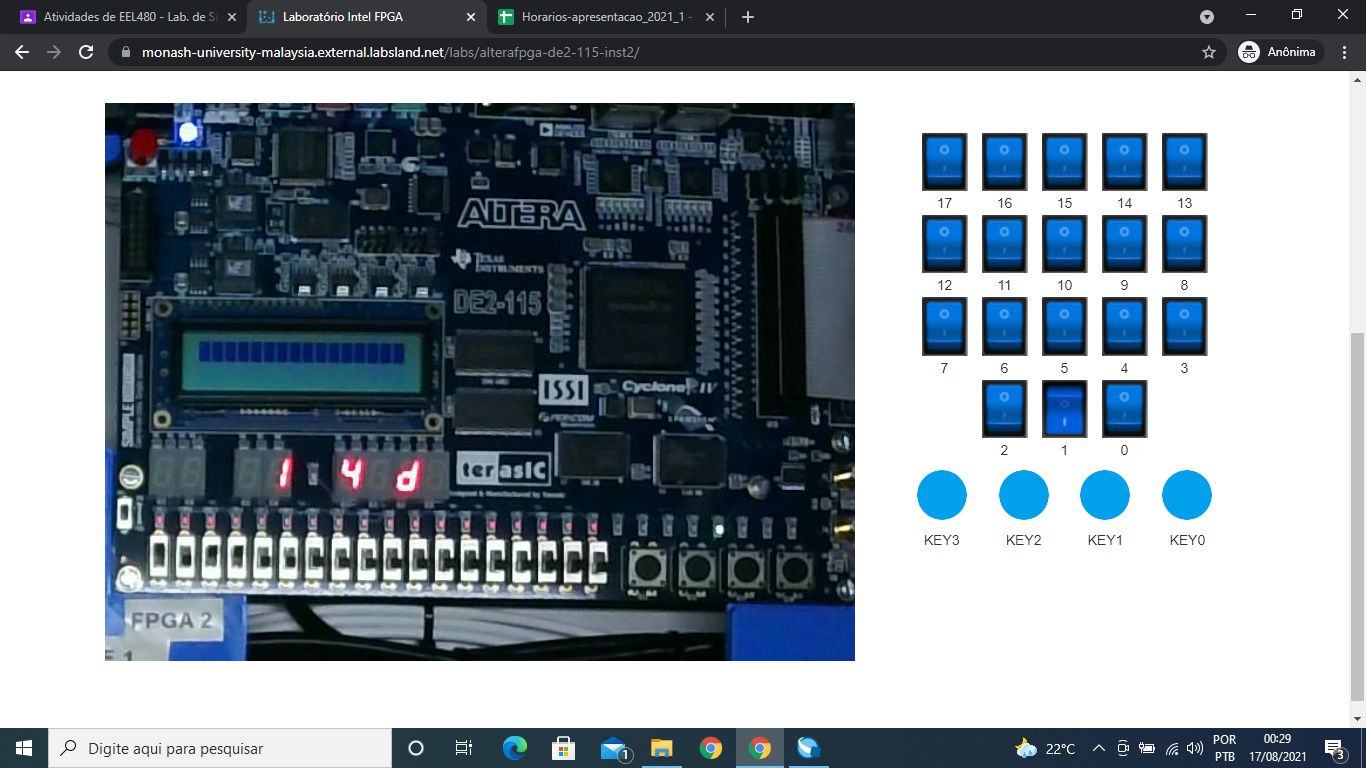
\includegraphics[width=\textwidth]{img/labsland_subtracao.png}
\caption{Subtração: 1 - 4 = d (-3). Note a flag de negativo acessa (4 led
    partindo da direita para a esquerda)}
\end{figure}

\end{center}

\section{Conclusão}

    Dadas as especificações, o projeto funcionou como esperado na placa física do
Labsland. O método de desenvolver um projeto o mais modularizado possível provou-se
bastante efetivo, pois permitiram testes contínuos no Quartus, que logo acusavam
as falhas e inconsistências no código, quando haviam. E esse aspecto foi notadamente
importante pelo fato de ser um projeto implementado em uma linguagem (VHDL) e em um 
dispositivo (FPGA) com os quais eu não possuía muita familiaridade.

O paradigma não convencional da linguagem VHDL me impôs uma curva de
aprendizado inicial, pois eu apenas havia tido experiência com linguagens de
programação, cujas instruções são sequenciais, não paralelas como neste caso.

\section{Referências bibliográficas}

[1] Ronald J. Tocci, Neal S. Widmer, Gregory L. Moss, "Sistemas Digitais: princípios e aplicações".

\end{document}
